\chapter{The CMS Detector} \label{chap:detector}

Particle accelerator is invited for artificially producing the hard collisions between particles to study not only the interaction between particles, but also probe the structure of the hadrons. The Large Hadron Collider (LHC) is the most power one that is still operating since 10 September 2008. It uses a multi-stage acceleration loops to boost proton or anti-proton beam reach to 6.5~TeV and collide two protons or anti-protons at the center-of-mass energy 13~TeV. Besides of the proton beam, it can also accelerates other type of ion beam and perform variety collisions such as proton-lead or lead-lead in lower center-of-mass energy per nucleon pair~\cite{Evans:2008zzb}.

\begin{figure}[ht]
  \begin{center}
    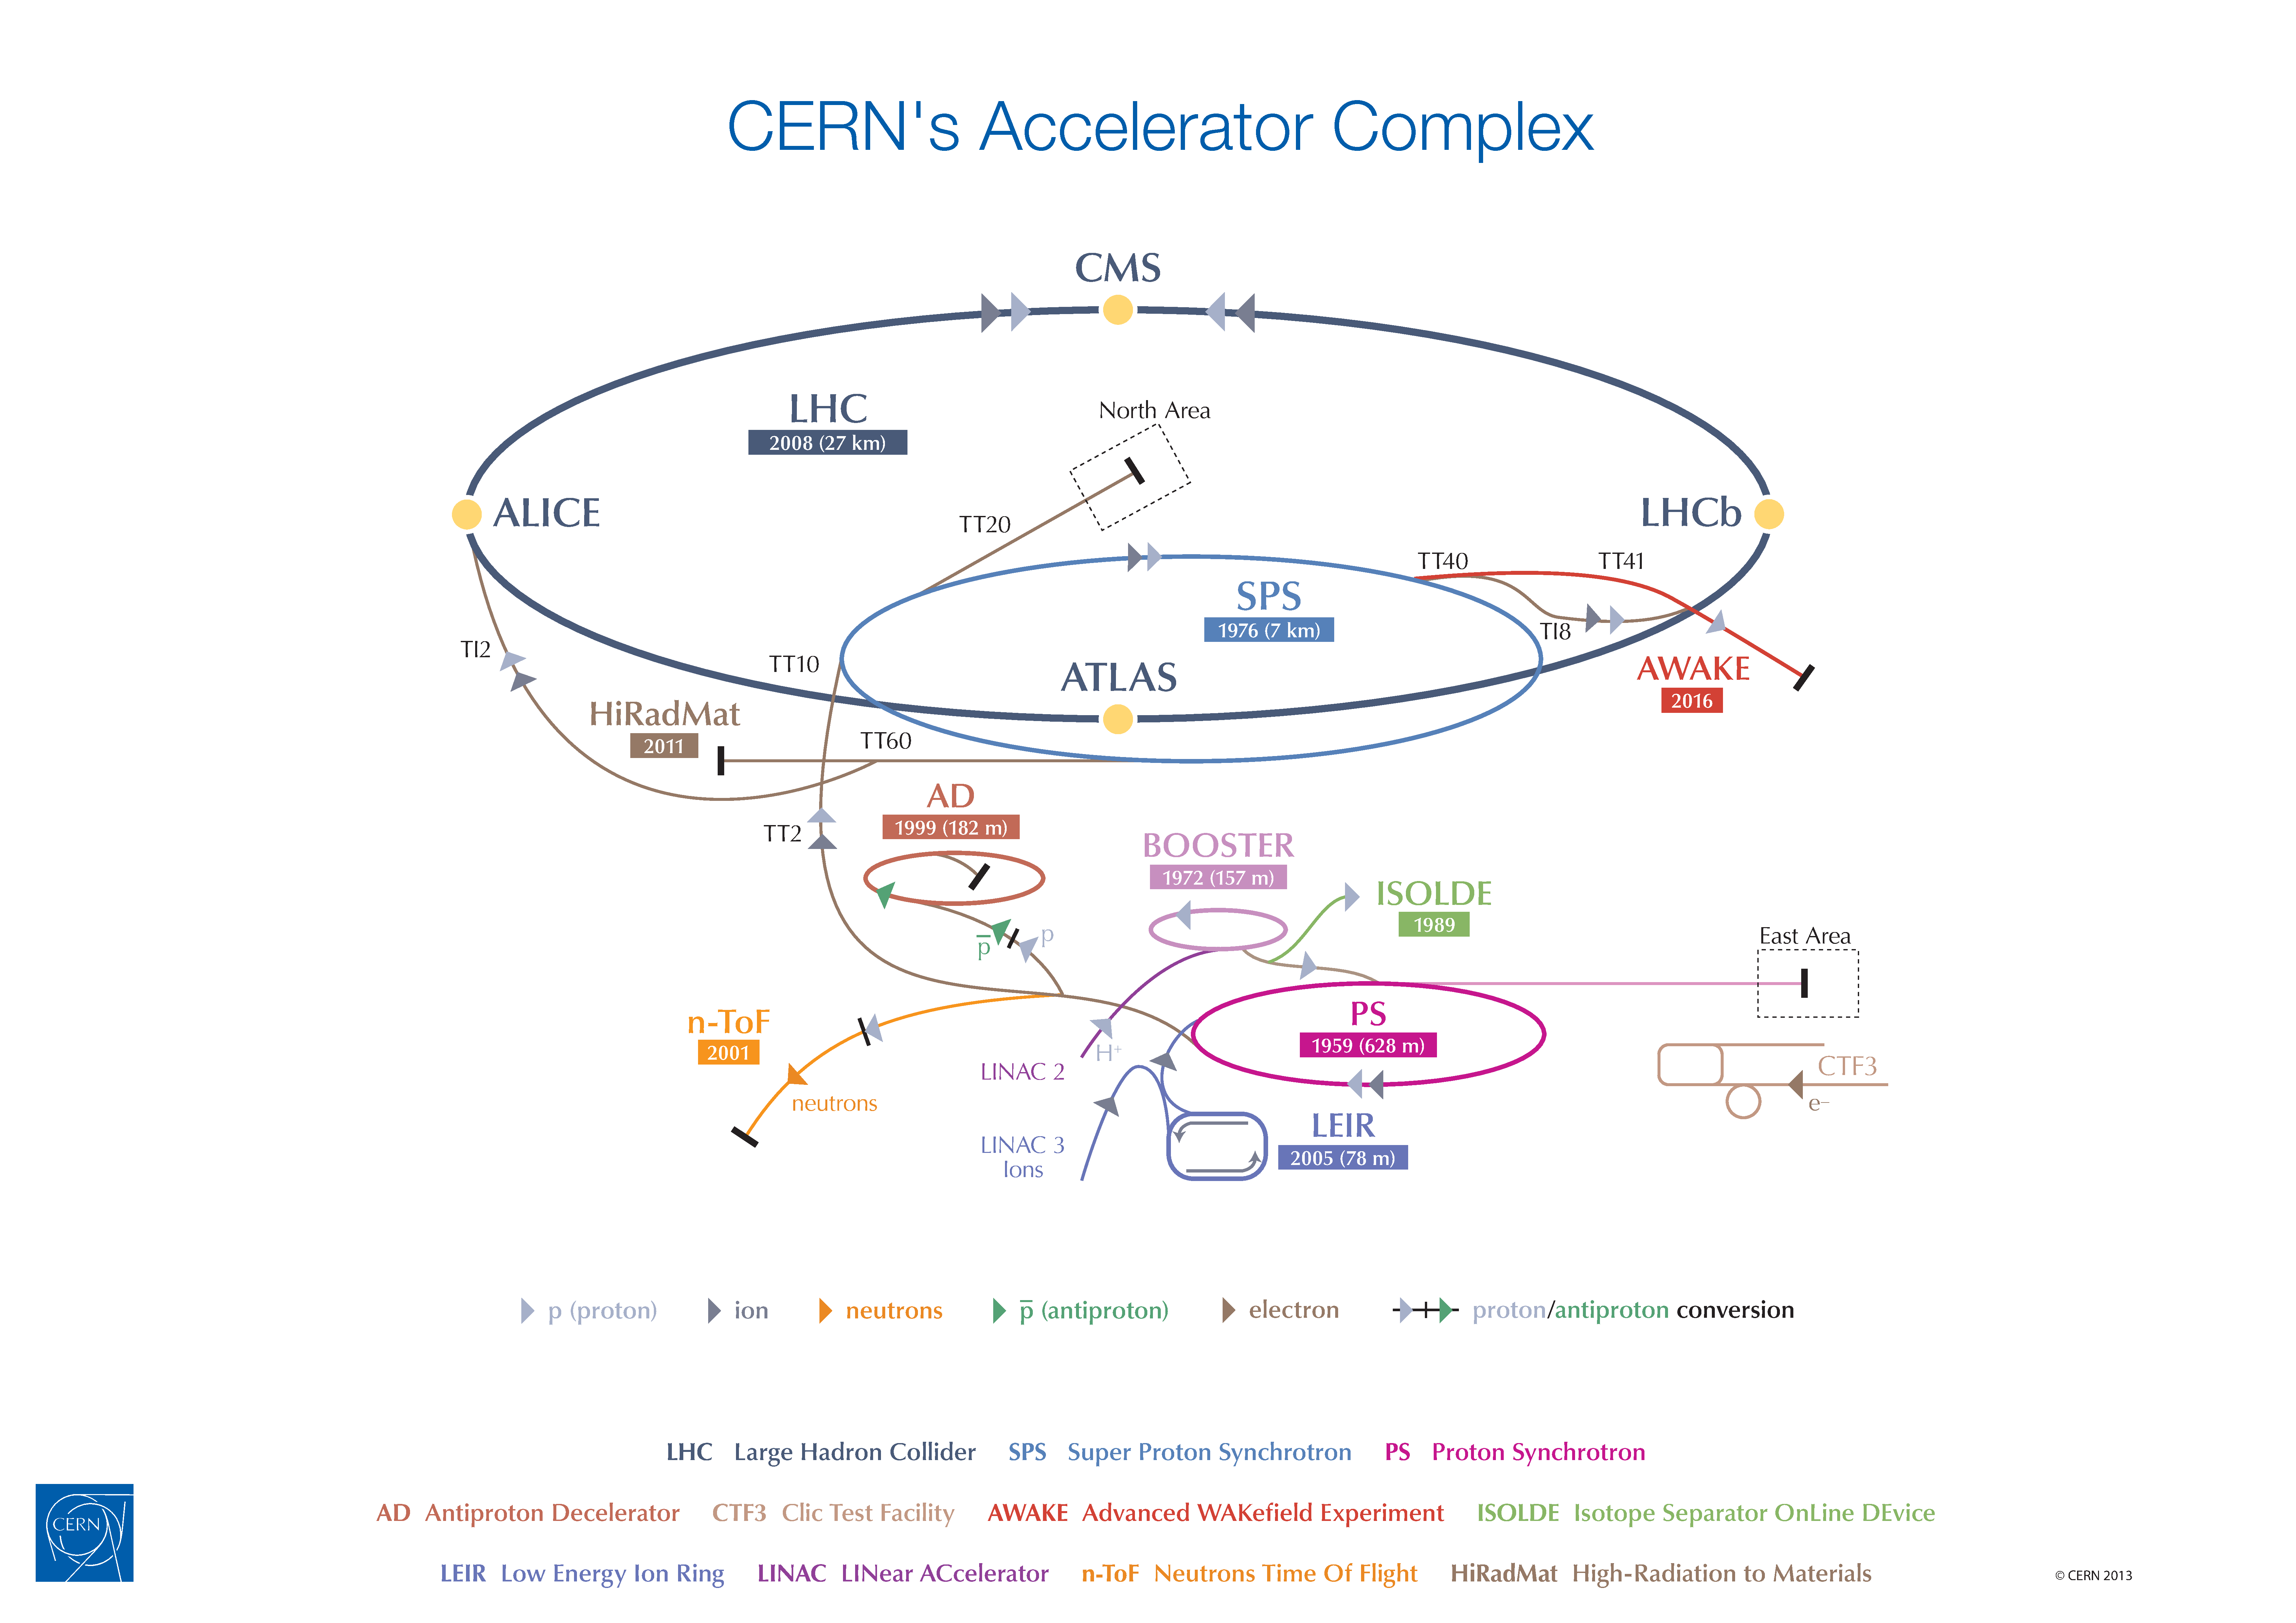
\includegraphics[width=1\textwidth]{figures/detector/LHC_complex_2013.pdf}
  \end{center}
  \caption{The schematic diagram of the LHC complex. Figure from CERN-Poster-2013-377.}
  \label{fig:lhc}
\end{figure}


There are four detectors mounted at each of the 4 beam crossing points: Compact Muon Solenoid (CMS), A Toroidal LHC ApparatuS (ATLAS), Large Hadron Collider beauty (LCHb) and A Large Ion Collider Experiment (ALICE). The CMS and ATLAS are general purpose detector while the ALICE and LHCb are designed to specific experiments. 

The LHC delivered proton beams reached the peak instance luminosity about $2.1\times 10^{34}$~cm$^2$s$^{-1}$ in Run2. And reached three and a half more than designed luminosity in 2015 lead-lead collisions with a peak instance luminosity of $2.7\times10^{27}$~cm$^2$s$^{-1}$. LHC delivered 1.88~nb$^{-1}$ inn 2018 lead-lead collisions at $\sqrt{s_{\text{NN}}}=5.02$~TeV and CMS detector received 1.78~nb$^{-1}$ with a peak instance luminosity of $6.4$ Hz$/$mb. With the high instance luminosity, several hard collisions may happen in one bunch cross and this phenomenon is called "pileup"~\cite{Sirunyan:2020foa}. The number of the hard collisions per bunch crossing can reach about 60 in high luminosity proton run. However, the pileup is keeping very low in PbPb collisions due the particle multiplicity can be very high in PbPb hard collisions.

The CMS detector is a versatile particle detector consists by several sub-detectors: a pixel and strip based tracking system, a calorimeter system combined by a electromagnetic calorimeter (ECal) followed by a hadronic calorimeter (HCal), and a superconducting solenoid magnet followed by muon detectors. The perspective of the CMS detector is illustrated in the Fig.~\ref{fig:cms_perspective}. The schematic diagram of the trajectory of different types of particles traveling through the CMS detector is illustrated in the Fig.~\ref{fig:cms_trajectory}.

\begin{figure}[ht]
  \begin{center}
    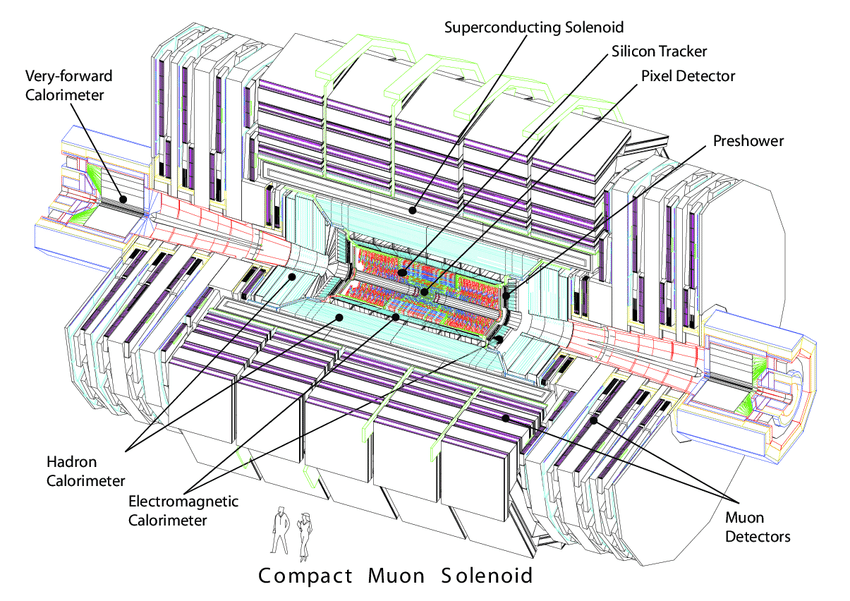
\includegraphics[width=0.7\textwidth]{figures/detector/cms_detector_prespective.png}
  \end{center}
  \caption{The perspective view of the CMS detector~\cite{Chatrchyan:2008aa}.}
  \label{fig:cms_perspective}
\end{figure}

\begin{figure}[ht]
  \begin{center}
    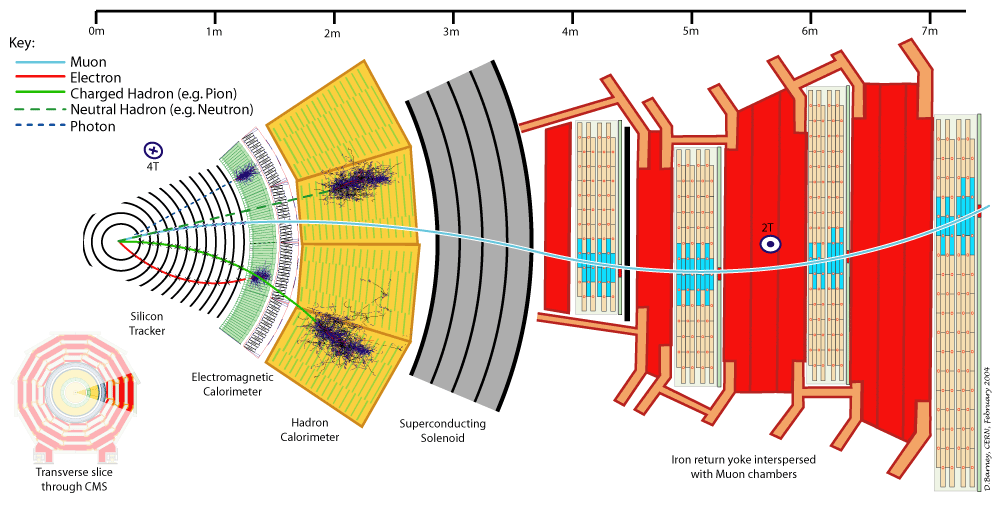
\includegraphics[width=1\textwidth]{figures/detector/CMS_particle_trajectory.png}
  \end{center}
  \caption{The schematic diagram of the particle trajectory traveling through the CMS detector.}
  \label{fig:cms_trajectory}
\end{figure}

\section{The CMS Tracker}
The CMS tracker consists by a inner silicon pixel detector covered by a silicon strip detector. The original configuration of the tracker is illustrated in the Fig.~\ref{fig:cms_tracker}. A right-handed coordinate is used in the CMS tracker. The origin point is at the collision point, $x$-axis points to the center of the LHC ring, a the $y$-axis pointing to the sky, and $z$-axis pointing to the anti-clockwise beam direction. The azimuthal angle $phi$ measured in the $x$-$y$ plane with $\phi=0$ refers to the $x$-axis. 

The three concentric cylindrical barrel pixel layers are arranged at 4.3, 7.3 and 10.2 cm in radius away from the beam while the two forward pixel disks are placed at each side where $z=\pm35.5$ and $z=\pm48.5$~cm away from the collision points. One more layer is added to barrel and each side of forward after the phase-1 upgrade finished in 2017~\cite{TrackerGroupoftheCMS:2020bgg}. This pixel detector is designed to provide a high precision three dimensional information of points left by the charged particle traveling through the silicon pixel. The barrel pixel provides a 4-hit efficient coverage in the region $|\eta|<2.2$ and the forward pixel provides a 3-hit efficient coverage in the region $|\eta|<2.5$. A 3.8~T magnetic field imposes a significant Lorentz force bending the charged particle trajectory to provides a better resolution for particles with different charge-to-mass ratio.

\begin{figure}[ht]
  \begin{center}
    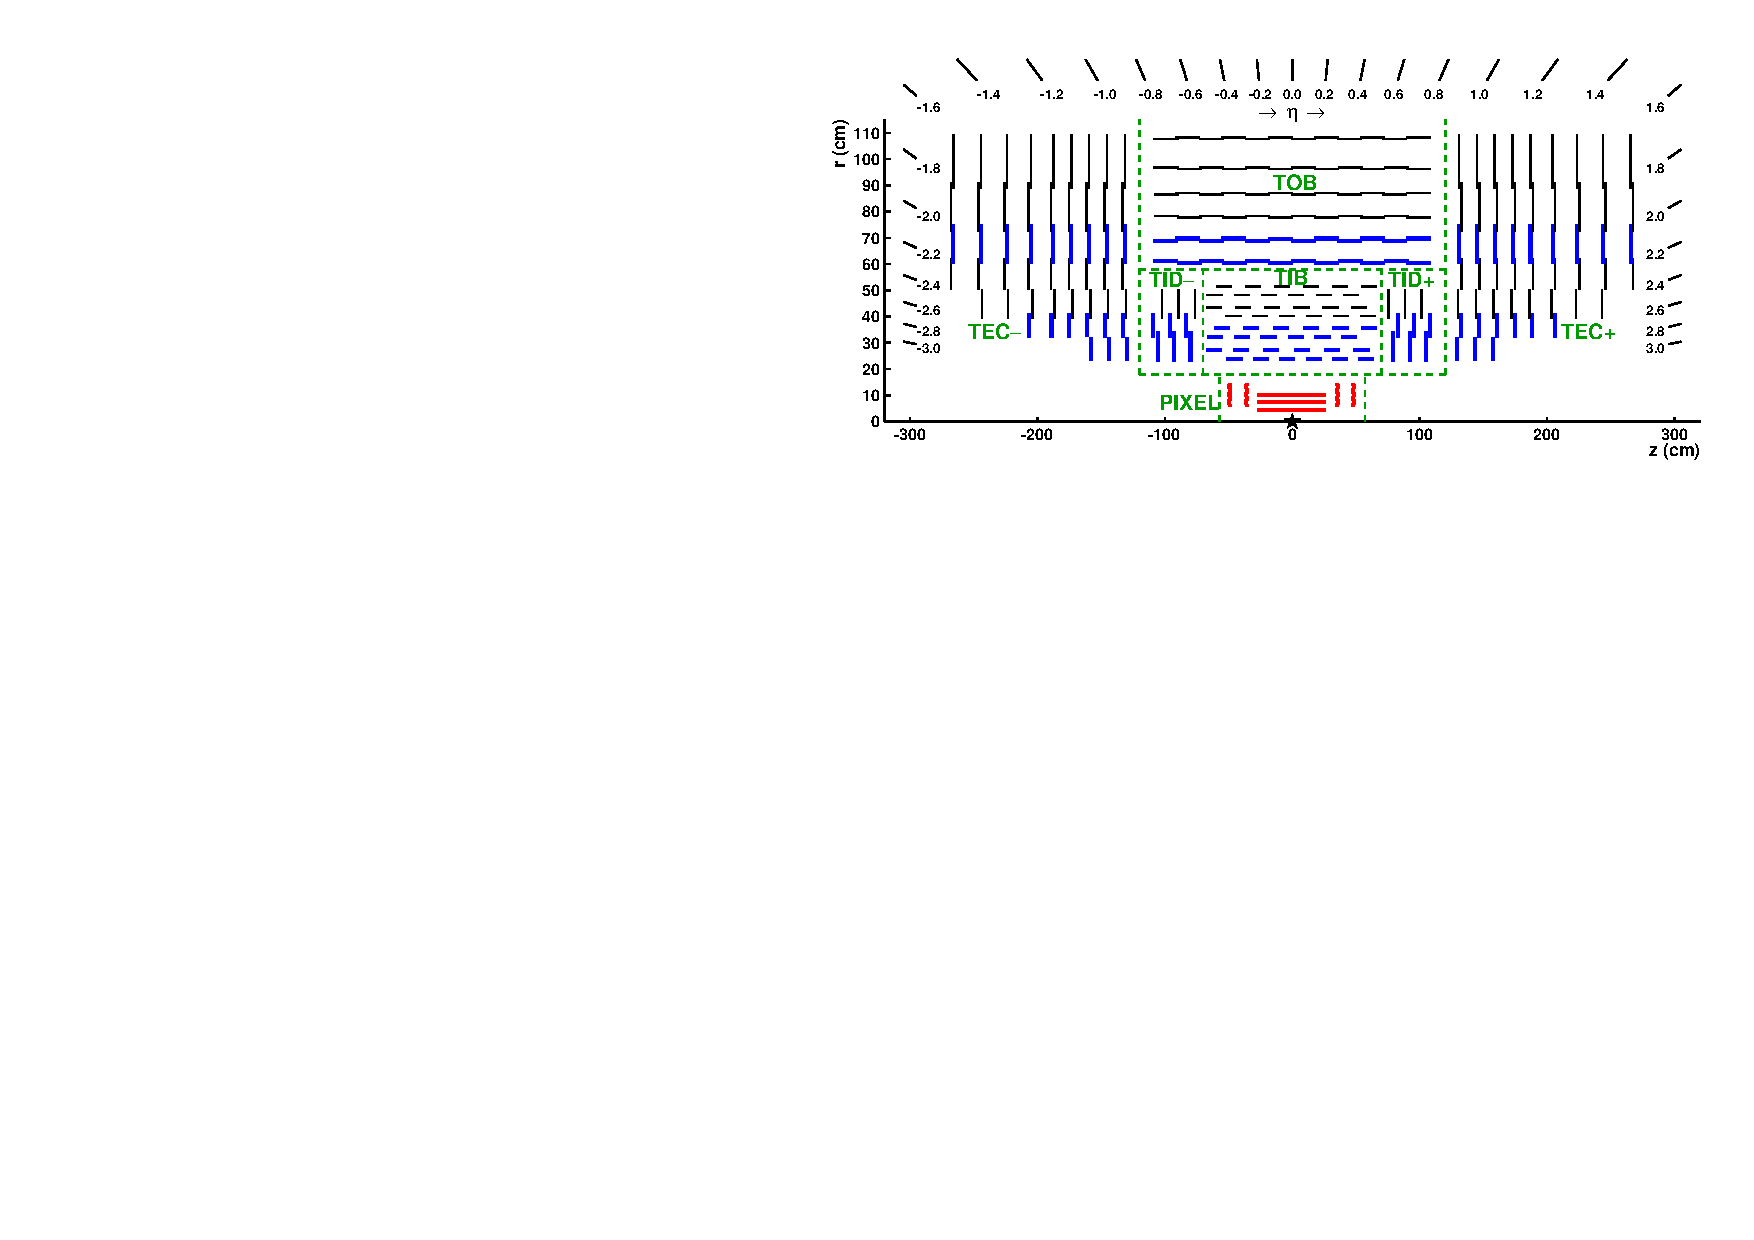
\includegraphics[width=0.8\textwidth]{figures/detector/TrackerLayoutNew.pdf}
  \end{center}
  \caption{The schematic diagram of the positions of CMS tracker layers and disks in a $z-r$ plane. The blue lines refer to the "stereo" modules and the red lines are pixel layers and disks. Figure from~\cite{Chatrchyan:2014fea}}
  \label{fig:cms_tracker}
\end{figure}

The CMS silicon strip detector is installed outside of the pixel detector. This strip detector consists by three major components: a Tracker Inner Barrel and Disk (TIB/TID) composed by 4 barrel layers and 3 forward disks, a Tracker Outer Barrel (TOB) consists of 6 layers and a Tracker EndCap (TEC) with 9 disks. The TIB strips placed parallel to the z direction and the disks of TID placed perpendicular to the z-axis can provides up to 4 $r$-$\phi$ measurements on one trajectory. The TIB/TID is surrounded by the TOB extended to 116~\cm in radius, and $\pm118$~cm in $z$ direction. The disks of TEC are placed in the region $124<|z|<280$~cm on each side of TOB. Considering hits counted from stereo modules, the strip detector can provides from 8 to 14 efficient measurements of track impact points in the region $|\eta|<2.4$~\cite{CMS:2010yua}.

\section{The CMS Calorimeter Detector}

The calorimeter detector is designed to absorb all the incident particle energy so that it can provide efficient position and the energy information for those particles. The incident particles will interact with the material of calorimeter and shower cascades of secondary particles until all the energy has been absorbed by the material. The particles can be stopped by either electromagnetic interaction which cause the electromagnetic shower, or scattering from nucleons which cause the hadronic shower. The Electromagnetic Calorimeter (ECAL) and the Hadronic Calorimeter (HCAL) are designed to handle the two types of showers, separately. 


\subsection{Electromagnetic Calorimeter}
ECAL placed outside of the CMS tracker is combined by a cylinder barrel consisted by a matrix of 61,200 PbWO$_4$ crystals and two flat "endcaps" sealed the two end side of barrel by about 15,000 extra crystals. The ECal barrel (EB) with crystal size $22\times 22$~mm$^2$ in $\eta-\phi$ plane and $23$~cm in depth provides a $1^\circ$ azimuthal granularity covering the region $|\eta|<1.48$ while the ECal Endcaps (EE) cover the forward region $1.48<|\eta|<3.0$ by disks arranged $29\times29$~mm$^2$ crystal~\cite{Bayatian:2006nff}. Further more, a preshower (ES) detector made by lead and silicon sensors is placed in front of the ECAL EE to distinguish neutral pions in close spatial proximity, which usually decay into two photons. A schematic view of the CMS ECAL is shown in Fig.~\ref{fig:cms_ecal}

\begin{figure}[ht]
  \begin{center}
    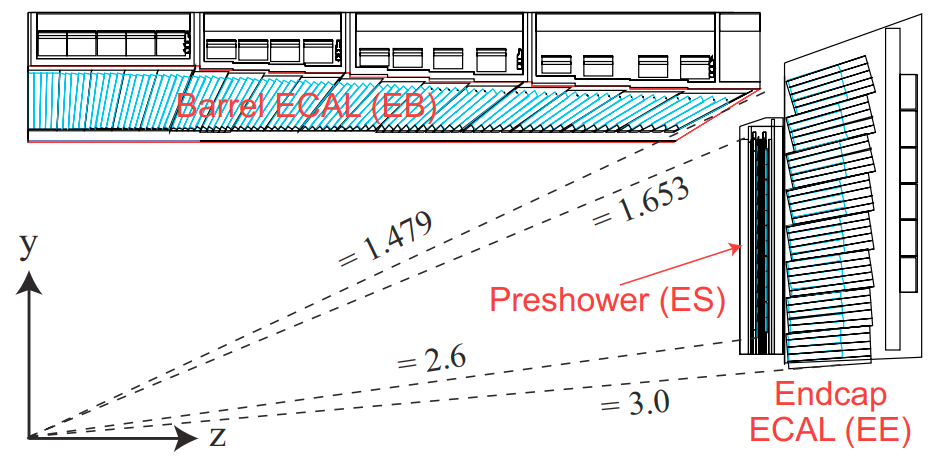
\includegraphics[width=0.8\textwidth]{figures/detector/CMS_ECAL.png}
  \end{center}
  \caption{The schematic view of the CMS ECAL in $y-z$ plane~\cite{Bayatian:2006nff}.}
  \label{fig:cms_ecal}
\end{figure}

The PbWO$_4$ that stopping the electrons and photon mainly through the bremsstrahlung and pair production, respectively, has a radiation length 0.89~cm which corresponds to a 2.2~cm Moliere radius. The 23~cm length (about 25.8 times of the radiation length) of PbWO$_4$ crystal can absorb approximately $98\%$ of depth of particles showered from 1~TeV electrons. Associating the signal from adjusted crystals, the position of the high energy electrons can be determined in an accuracy of $0.5$~mm, which allows matching the shower positions with the tracks reconstructed from the CMS tracker. However, the transparency of the crystal will decrease due to the thermal damage and irradiation dose it took. This makes the ECAL to be a destructive detector and the energy response of the ECAL is calibrated periodically using the laser beam. The energy resolution of ECAL can be parameterized as
\begin{equation}
	\left(\frac{\sigma}{E}\right)^2=\left(\frac{S}{\sqrt{E}}\right)^2+\left(\frac{N}{E}\right)^2+C^2,
\end{equation}
where the $S,N,C$ stands for the stochastic, noise and constant term, respectively. For electrons with energy below 500~MeV, the resolution estimated by using a matrix of $3\times3$ crystals is parameterized as
\begin{equation}
	\left(\frac{\sigma}{E}\right)^2=\left(\frac{2.8\%}{\sqrt{E}}\right)^2+\left(\frac{0.12}{E}\right)^2+(0.30\%)^2,
\end{equation}
where $E$ is in GeV~\cite{Chatrchyan:2008aa}. 


\subsection{Hadronic Calorimeter}
The CMS HCAL is a sampling calorimeter designed to measure the hadron energy by stopping and absorbing hadronic cascade showers produced from the incident hadrons. It lies between the ECAL and the CMS solenoid, and consists by four sub-detectors: the Hadronic Barrel (HB), Hadronic Endcap (HE), Hadronic Outer (HO) and Hadronic Forward (HF) calorimeters. The HB composed by  18 wedges, each cover $20^\circ$ in $\phi$, placed outside of the ECAL barrel to cover the $|\eta|<1.4$ region. Each of the HB wedges  covered by stainless steel uses 18 layers of brass as absorber interleaved with 17 plastic scintillator. The HO is made by brass disks, interleaved with scintillators which cover $20^\circ$ in $phi$ to cover forward region $1.3<|\eta|<3.0$. The thickness of HB at $\eta=0$ is about 5.8 hadronic interaction length and increase to 10 interaction length at $|\eta|= 1.2$. Each segment of the HCAL is aligned to a $5\times5$ crystal matrix in ECAl. The HB and HE calorimeters have granularity $\Delta\eta\times \Delta\phi=0.087\times0.087$ for the region $|\eta|<1.6$ and $\Delta\eta\times \Delta\phi=0.175\times0.175$ for the region $1.6<|\eta|<3.0$. Energy leakage from HB and HE is supposed by captured by the HO consisted by 12-fold scintillator layers.

\begin{figure}[ht]
  \begin{center}
    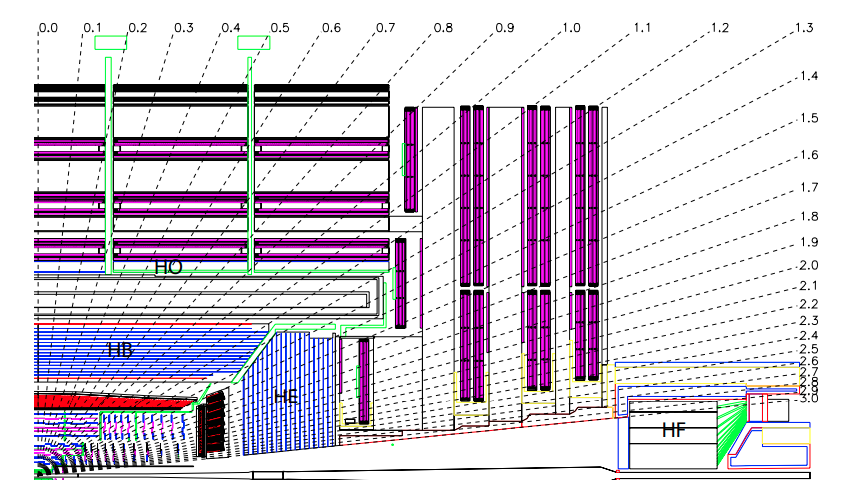
\includegraphics[width=0.8\textwidth]{figures/detector/CMS_HCAL.png}
  \end{center}
  \caption{The schematic view of the CMS HCAL in $y-z$ plane~\cite{Bayatian:2006nff}.}
  \label{fig:cms_hcal}
\end{figure}

The HF extends the calorimeter to a very space like proximity region $3.0<|eta|<5.0$ where enormous radiation fluences shade on, typically in a Grad dose level. It consists by steel absorber and the quartz fiber Cherenkov Calorimeters which utilize the Cherenkov radiation produced by the shower charged particles in fiber to measure the energy of those electromagnetic showers. The advantage of this design is not only the quartz fiber tolerates to this high dose of radiation, but also the Cherenkov radiation is produced essentially simultaneously to makes a fast response in HF. The HF is a cylindrical steel structure with length 165~cm, outer radius 130~cm and inner radius 12.5~cm. There are 18 absorber wedges, each one covers 20 degree in azimuthal angle, placed in each side of the CMS interaction point. The two sizes of quartz fibers are alternate in nearby grooves space by 5~mm inserted into the absorber parallel to the $z$ direction: a short length fiber only go through the first 22~cm from the front of the absorber while the long length fiber go all the way through the absorbers. This arrangement allows the HF to distinguish the electromagnetic shower energy from the hadronic showers since electrons and photon typically starts shower at a relatively long depth in the absorber and hence leaves signal mainly on long fibers while the signal of hadronic showers can be detected in both length of fibers~\cite{Penzo:2009zz}. The HF segmentation is $0.175\times0.175$ for $|\eta|<4.7$ and $0.175\times0.35$ for $|\eta|>4.7$~\cite{Chatrchyan:2009ag}. The schematic organization of the HB, HE, HO and HF is shown in Fig.~\ref{fig:cms_hcal}.
	

\section{The CMS Trigger System}
The collision rate delivered by LHC can reach 1~GHz. With an estimation of about 1~MeV per event record, it is not practice to store all the events for analyzing. Therefore, a two-stage sophisticated trigger system is used to promptly identify the interest event to recording. The first staged is a hardware based Level 1 Trigger (L1) and multiple software-based High-Level Triggers (HLT) form the second stage. The architecture of the CMS trigger system is illustrated in Fig.~\ref{fig:cms_trigger}. 

\begin{figure}[ht]
  \begin{center}
    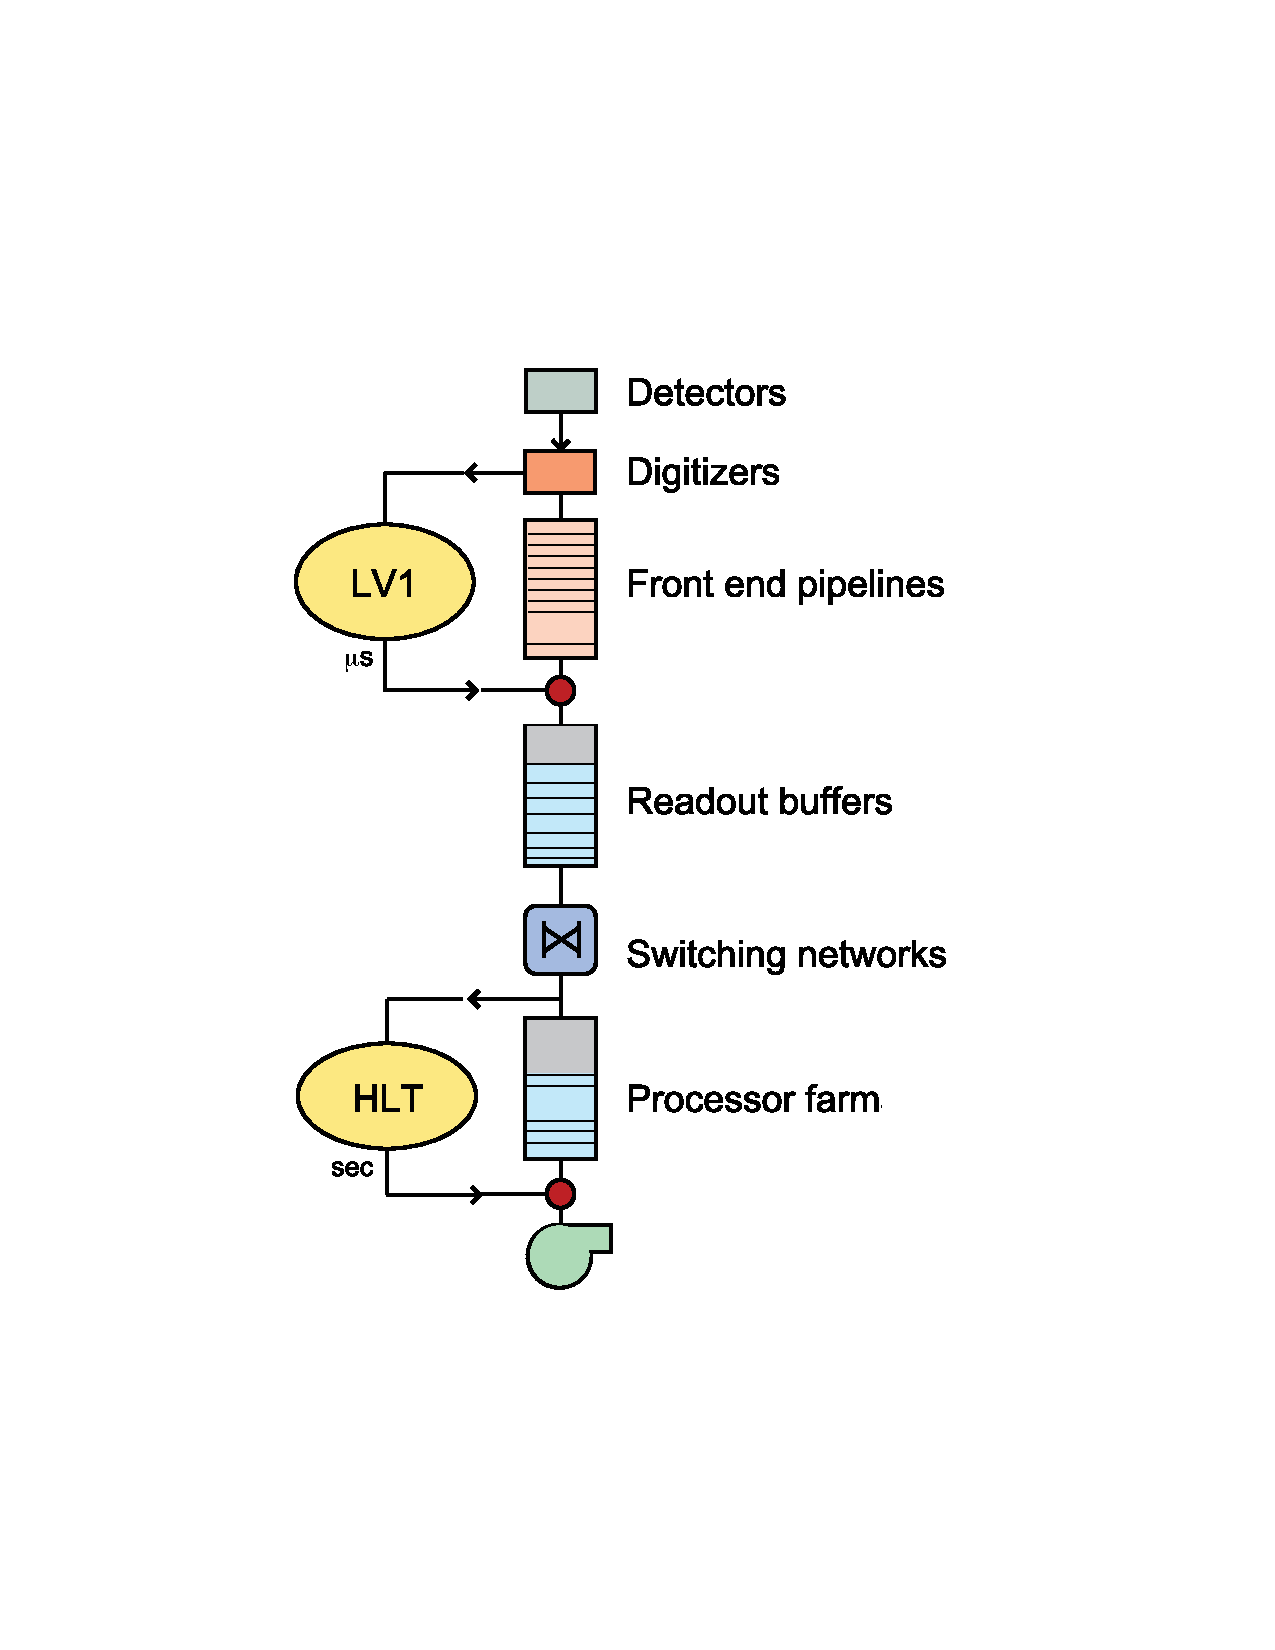
\includegraphics[width=0.5\textwidth]{figures/detector/CMS_Trigger.pdf}
  \end{center}
  \caption{The schematic diagram of the CMS trigger system~\cite{Chatrchyan:2009ic}.}
  \label{fig:cms_trigger}
\end{figure}

The L1 which made out of Filed-Programmable Gate Arrays (FPGAs) and Application Specific Integrated Circuits (ASICs) to limit the latency within $1$~$\mu$s for response is designed to reduce the event rate to 100~kHz at the LHC designed instance luminosity $\mathcal{L}=10^{34}$~cm$^2$s$^{-1}$. The total latency of the L1 is fixed at $3.2$~$\mu$s as the signal transition consumes a lot of time. Therefore the L1 system uses coarser granularity and lower resolution information (comparing to the signal from the front-end-electronics) from the calorimeters and muon chambers to search the energy deposit or hits for deciding whether this event should be kept. The full event information from front-end-electronics stand-by in pipelines will be collected and send to readout buffer once the the L1 selected the event. A switching network will distribute the data from readout to the HLT computing nodes (known as "Event Filter Farm") which are PCs mounting 2.66~GHz dual quad-core Intel processors accomplish with 16~GB RAM. The HLT algorithm is the modified offline reconstruction algorithm, which has improved processing speed, to produce high level physics object, like tracks and jets, for precisely identifying the event of interests and further reducing the event rate to the order of 100~Hz. 

The event data selected from different HLTs will be streamed to corresponding dataset. However, due to the recording bandwidth limitation, not all events past the L1+HLT can be kept. A prescale scheme is adapted to feasibly adjust the fraction of events selected from different HLTs: a HLT with a prescaled rate $n$ implies that one event will be recorded for every $n$ events past this HTL. The events with the prescale number 1 is called unprescaled events. The final survived event will be store and reconstructed in offline computing center. The raw data and the reconstruction output will be transfered to the data center for long term storage.  